\documentclass{article}
\usepackage{graphicx}
\graphicspath{ {Announcements/} }
\usepackage{hyperref}
\usepackage[margin=0.5in]{geometry}

\begin{document}

\section*{How to Make Changes to the SFUCSSS Website}

\subsection*{Before Making Any Changes...}
\begin{enumerate}
	\item Go to \url{sfucsss.org/admin} in your browser
	\item Use the page to Login to the Admin Control Panel (Note: You will need a valid set of Admin credentials in order to Login)
	
\end{enumerate}

\subsection*{How to Create a Front-Page Announcement}
\begin{enumerate}
	\item Under the "Site Administration" heading, find the "Cms" sub-heading
	\item Under the "Cms" sub-heading, find the Announcements row
	\item Click on the "Add" button on the right-hand side of the Announcements row
	
	\includegraphics[scale=0.45]{Announcements-picture1.png}
	
	\item Fill in all relevant information for the announcement
	\item Save the announcement
	
\end{enumerate}

\subsection*{How to Modify or Delete an Existing Front-Page Announcement}
\begin{enumerate}
	\item Under the "Site Administration" heading, find the "Cms" sub-heading
	\item Under the "Cms" sub-heading, find the Announcements row
	\item Click on the "Change" button on the right-hand side of the Announcements row
	
	\includegraphics[scale=0.45]{Announcements-picture2.png}
	
	\item Click on the name of the announcement you wish to modify or delete
	\item Modify any information for the announcement, then save your edits
	
	\textbf{OR}
	
	Delete the announcement

\end{enumerate}

\subsection*{How to Create a Toolbar Category}
\begin{itemize}
	\item Example Categories: 
	
	\includegraphics[scale=0.45]{Categories-picture1.png}
	
\end{itemize}
\begin{enumerate}
	\item Under the "Site Administration" heading, find the "Cms" sub-heading
	\item Under the "Cms" sub-heading, find the Categories row
	\item Click on the "Add" button on the right-hand side of the Categories row
	
	\includegraphics[scale=0.45]{Categories-picture2.png}
	
	\item Fill in all relevant information for the category
	\item Save the category
	
\end{enumerate}

\subsection*{How to Modify or Delete an Existing Toolbar Category}
\begin{enumerate}
	\item Under the "Site Administration" heading, find the "Cms" sub-heading
	\item Under the "Cms" sub-heading, find the Categories row
	\item Click on the "Change" button on the right-hand side of the Categories row
	
	\includegraphics[scale=0.45]{Categories-picture3.png}
	
	\item Click on the name of the category you wish to modify or delete
	\item Modify any information for the category, then save your edits
	
	\textbf{OR}
	
	Delete the category
	
\end{enumerate}

\subsection*{How to Create a Page}
\begin{enumerate}
	\item Under the "Site Administration" heading, find the "Cms" sub-heading
	\item Under the "Cms" sub-heading, find the Posts row
	\item Click on the "Add" button on the right-hand side of the Posts row
	
	\includegraphics[scale=0.45]{posts-picture1.png}
	
	\pagebreak
	
	\item Fill in all relevant information for the page (Note: The information in coloured boxes in the image is required to create the page)
	
	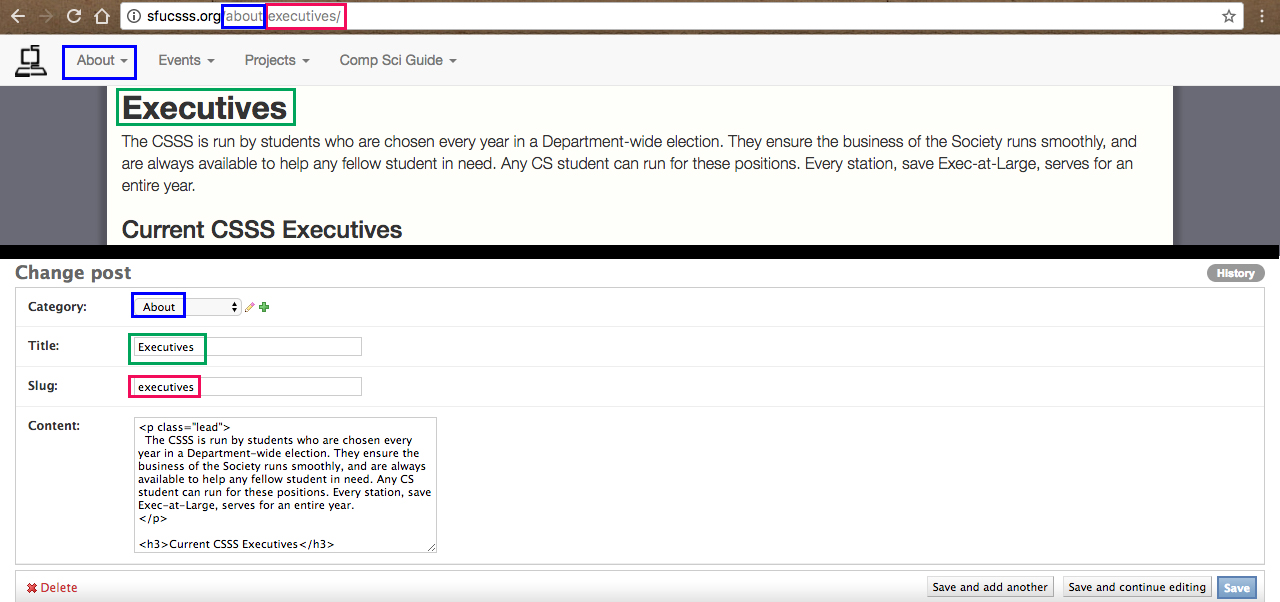
\includegraphics[scale=0.40]{Posts.jpg}
	
	\item Save the page
	
\end{enumerate}

\subsection*{How to Modify or Delete an Existing Page}
\begin{enumerate}
	\item Under the "Site Administration" heading, find the "Cms" sub-heading
	\item Under the "Cms" sub-heading, find the Posts row
	\item Click on the "Change" button on the right-hand side of the Posts row
	
	\includegraphics[scale=0.45]{posts-picture2.png}
	
	\item Click on the name of the page you wish to modify or delete
	\item Modify any information for the page, then save your edits
	
	\textbf{OR}
	
	Delete the page
	
\end{enumerate}

		
\end{document}